% diagrams/english/habitacion.tex -- el cuarto de Lucía, para "Where is
% it?": la cama debajo de la ventana (con patas, para que quepa algo
% debajo), la estantería de libros al lado, y el escritorio con su silla.
% Se dibujan encima las cosas que dice el texto.
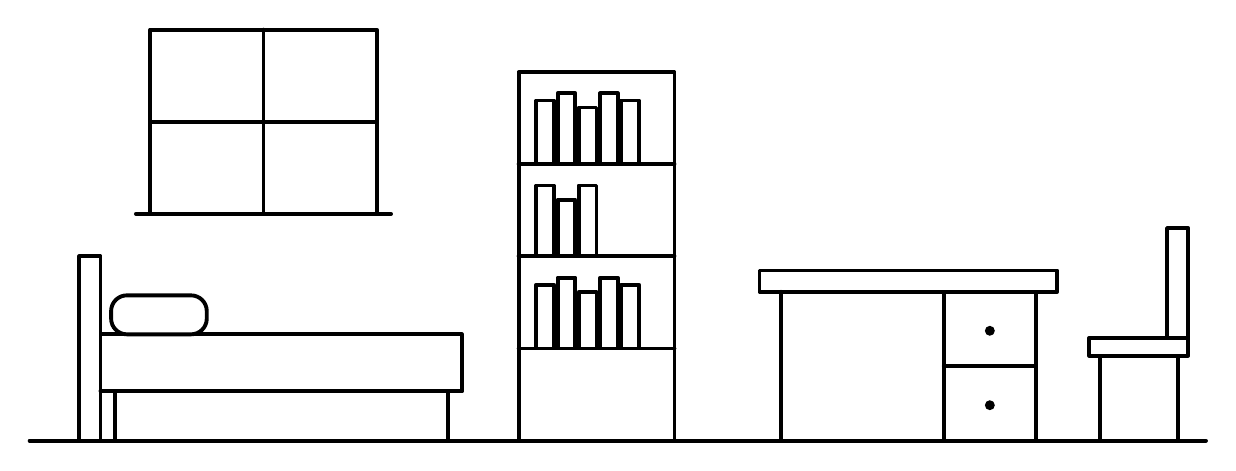
\begin{tikzpicture}[line width=1.4pt, line cap=round, line join=round, scale=0.9]
  % suelo y pared
  \draw (-0.3,0) -- (16.3,0);
  % la ventana
  \filldraw[fill=white] (1.4,3.2) rectangle (4.6,5.8);
  \draw (3.0,3.2) -- (3.0,5.8); \draw (1.4,4.5) -- (4.6,4.5);
  \draw (1.2,3.2) -- (4.8,3.2);
  % la cama, debajo de la ventana
  \filldraw[fill=white] (0.4,0) rectangle (0.7,2.6);
  \draw (0.7,0.7) -- (5.8,0.7);
  \filldraw[fill=white] (0.7,0.7) rectangle (5.8,1.5);
  \draw (5.6,0.7) -- (5.6,0); \draw (0.9,0.7) -- (0.9,0);
  \filldraw[fill=white, rounded corners=2mm] (0.85,1.5) rectangle (2.2,2.05);
  % la estantería, al lado de la cama
  \filldraw[fill=white] (6.6,0) rectangle (8.8,5.2);
  \foreach \y in {1.3,2.6,3.9} { \draw (6.6,\y) -- (8.8,\y); }
  \foreach \x/\h in {6.85/0.9,7.15/1.0,7.45/0.8,7.75/1.0,8.05/0.9} {
    \draw (\x,1.3) rectangle ++(0.25,\h);
    \draw (\x,3.9) rectangle ++(0.25,\h);
  }
  \foreach \x/\h in {6.85/1.0,7.15/0.8,7.45/1.0} { \draw (\x,2.6) rectangle ++(0.25,\h); }
  % el escritorio, con sus cajones, y la silla
  \filldraw[fill=white] (10.0,2.1) rectangle (14.2,2.4);
  \draw (10.3,2.1) -- (10.3,0);
  \filldraw[fill=white] (12.6,0) rectangle (13.9,2.1);
  \draw (12.6,1.05) -- (13.9,1.05);
  \fill (13.25,1.55) circle (0.07); \fill (13.25,0.5) circle (0.07);
  \draw (14.8,0) -- (14.8,1.2); \draw (15.9,0) -- (15.9,1.2);
  \filldraw[fill=white] (14.65,1.2) rectangle (16.05,1.45);
  \filldraw[fill=white] (15.75,1.45) rectangle (16.05,3.0);
\end{tikzpicture}
